\icode{E-MI-SI-L3-261104-004}
两个相同的小球由轻质细绳连接悬挂起来，\(O\)为悬挂点，现在对小球\(B\)施加一拉力（图中未画出），使\(OA\)段细绳偏离竖直方向的角度为\(\theta_1\)，使\(AB\)段细绳偏离竖直方向的角度为\(\theta_2\)。已知两球的质量均为\(m\)，虚线\Rmnum{1}与细绳\(AB\)段垂直，虚线\Rmnum{2}与细绳\(OA\)段垂直，虚线\Rmnum{3}沿水平方向，虚线\Rmnum{4}沿\(AB\)方向。不考虑其他外力，若要使对\(B\)球施加的拉力最小，则此拉力\paren[]

\begin{tikzpicture}[font=\scriptsize]
	\draw[magenta] (0,0)--(-60:1.5)coordinate(A)--++(-40.89:1.5)coordinate(B);
	\draw[dashed,cyan] (B)--++(49.01:1.5)node[above]{\Rmnum{1}} (B)--++(30:1.5)node[right]{\Rmnum{2}} (B)--++(0:1.5)node[right]{\Rmnum{3}} (B)--++(-40.89:1.5)node[right]{\Rmnum{4}};
	\draw[dashed,teal] (0,0)--(0,-2) (A)--++(-90:1.5);
	\shade[ball color=gray] (A)node[left]{\(A\)} circle(.1);
	\shade[ball color=gray] (B)node[below]{\(B\)} circle(.1);	
	\draw (0,-.3) arc(-90:-60:.3) ($(A)+(0,-.3)$) arc(-90:-40.89:.3);
	\node at(-.2,-.2){\(O\)};
	\node at(.2,-.7){\(\theta_1\)};
	\node at($(A)+(.25,-.5)$){\(\theta_2\)};
	\foreach \x in {-.8,-.6,...,.6}
		\draw[gray] (\x,.2)--++(.2,-.2);
	\draw[thick] (-.8,0)--(.8,0);
\end{tikzpicture}
\begin{choices}
	\item 方向沿虚线\Rmnum{1}，大小为\(mg\sin\theta_2\)
	\item 方向沿虚线\Rmnum{2}，大小为\(2mg\sin\theta_1\)
	\item 方向沿虚线\Rmnum{3}，大小为\(mg\tan\theta_2\)
	\item 方向沿虚线\Rmnum{4}，大小为\(2mg\sin\theta_1\)
\end{choices}
\begin{answer}
	B\qquad 提示：当外力\(F\)与\(OA\)垂直时，\(F\)最小。对\(A\)、\(B\)以及\(AB\)受力分析合并为下图

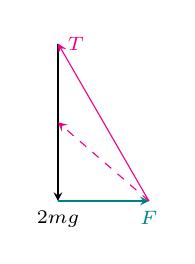
\begin{tikzpicture}[>=stealth,font=\scriptsize]
    \draw[->] (0,0)--(0,-2)node[below]{\(2mg\)};
    \draw[->,teal] (0,-2)--({2*sqrt(3)/3},-2)node[below]{\(F\)};
    \draw[->,magenta] ({2*sqrt(3)/3},-2)--(0,0)node[right]{\(T\)};
    \draw[->,dashed,magenta] ({2*sqrt(3)/3},-2)--(0,-1);
\end{tikzpicture}
\end{answer}